\documentclass[12pt, a4paper]{article}

% !TeX root = ../main.tex
\usepackage{a4wide}

\usepackage[utf8]{inputenc}

%\usepackage[ngerman]{babel}
\usepackage[english]{babel}

\usepackage[T1]{fontenc}
\usepackage{palatino}

\usepackage{graphicx}
\usepackage{caption}
\usepackage{url}
\usepackage{tocloft}
\usepackage{acronym}

\usepackage{mathpazo}
\usepackage{amsmath}
\usepackage{amsfonts}
\usepackage{adjustbox}

%\usepackage{subcaption}

\usepackage{hhline}
\usepackage{amssymb}
\usepackage{floatflt}
\usepackage{setspace}
\usepackage{float}
\usepackage{color}
\usepackage{listings}
\usepackage{array}
\usepackage{scrhack}
\usepackage{xcolor}
\usepackage{wrapfig}
\usepackage{hyperref}
\usepackage{url}
\usepackage{lmodern}
\usepackage{multirow}
\usepackage{subfig}
\usepackage{cleveref}
\usepackage{lipsum}


% !TeX root = ../main.tex
%%%%%%%%%%%%%%%%%%%%%%%%%%%%%%%%%%%%%%%%%%%%%%%%%%%%%%%%%%%%%%%%%%%%%%%%
% Data about you and the Document%
%%%%%%%%%%%%%%%%%%%%%%%%%%%%%%%%%%%%%%%%%%%%%%%%%%%%%%%%%%%%%%%%%%%%%%%%

% % Main Title of Document:
\newcommand{\myMaintitle}{Untersuchung und Aufbau einer DevOps Development Umgebung}

% % Sub Title of DocInput:
\newcommand{\mySubtitle}{Developing holistic software solutions through integration of existing individual solutions.}

% % Ihr Name:
\newcommand{\myName}{Henrik Gerdes}

% % Matrikelnummer:
\newcommand{\myMatrikel}{MatNr: 969272}

% % Ihr Geburtsort:
\newcommand{\brith}{Osnabrück}

% % Ihr Geburtsort:
\newcommand{\place}{Osnabrück}

% % Ihr Abgabedatum:
\newcommand{\submission}{\today}

% % Ihr Abgabedatum:
\newcommand{\mycourse}{Exposé für den B.Sc.}

% % Name des Betreuers/Erstprüfenden:
\newcommand{\fistSupervisor}{Dennis Ziegenhagen}
\newcommand{\secSupervisor}{Achim Hendrix}

% % In welchem Semester befinden Sie sich?
\newcommand{\mySemester}{6. Semester}

\title{\myMaintitle}

\author{\myName}
% !TeX root = ../main.tex
% % Zeilenabstand im Haupttext auf anderthalb-zeilig setzen
%\linespread{1.25}\selectfont

% Line spacing
%\onehalfspacing{}

%Pfad für Grafiken
\graphicspath{{fig/}}

%Styleregeln
\widowpenalty10000 % Vermeidet einzelne Zeilen eines Absatzes zu Beginn einer Seite
\clubpenalty10000 % Vermeidet einzelne Zeilen eines Absatzes am Ende einer Seite
\addtocontents{toc}{\protect\sloppy}
\setcounter{tocdepth}{3}


% % \sloppy bewirkt, dass Latex beim Blocksatz nicht über den rechten Rand hinausschreibt.
% % und dafür größere Lücken in einer Zeile in Kauf nimmt
\sloppy

% % Setzt Dokumenteigenschaften für PDFs, wenn das Paket 'hyperref' geladen wurde.
\hypersetup{pdftitle=\myMaintitle,pdfauthor=\myName,bookmarksopen=true}

%Source for picture captions
\newcommand{\source}[1]{\caption*{Source: {#1}} }

\newcommand{\code}[1]{\texttt{#1}}

\newcommand{\myparagraph}[1]{\paragraph{#1}\mbox{}\\}

\newcommand{\RM}[1]{\MakeUppercase{\romannumeral{} #1{}}}

\newcommand{\HRule}{\rule{\linewidth}{0.5mm}} % Defines a new command for horizontal


\definecolor{dkgreen}{rgb}{0,0.6,0}
\definecolor{gray}{rgb}{0.5,0.5,0.5}
\definecolor{mauve}{rgb}{0.58,0,0.82}

\lstset{ %
  language=Java,                  % the language of the code
  basicstyle=\footnotesize,       % the size of the fonts that are used for the code
  numbers=left,                   % where to put the line-numbers
  numberstyle=\tiny\color{gray},  % the style that is used for the line-numbers
  stepnumber=1,                   % the step between two line-numbers. If it's 1, each line
                                  % will be numbered
  numbersep=5pt,                  % how far the line-numbers are from the code
  backgroundcolor=\color{white},  % choose the background color. You must add \usepackage{color}
  showspaces=false,               % show spaces adding particular underscores
  showstringspaces=false,         % underline spaces within strings
  showtabs=false,                 % show tabs within strings adding particular underscores
  frame=single,                   % adds a frame around the code
  rulecolor=\color{black},        % if not set, the frame-color may be changed on line-breaks within not-black text (e.g. commens (green here))
  tabsize=4,                      % sets default tabsize to 2 spaces
  captionpos=b,                   % sets the caption-position to bottom
  breaklines=true,                % sets automatic line breaking
  breakatwhitespace=false,        % sets if automatic breaks should only happen at whitespace
  title=\lstname,                 % show the filename of files included with \lstinputlisting;
                                  % also try caption instead of title
  keywordstyle=\color{blue},          % keyword style
  commentstyle=\color{dkgreen},       % comment style
  stringstyle=\color{mauve}         % string literal style
}

%%%%%%%%%%%%%%%%%%%%%%%%%%%%%%%%%%%%%%%%%%%%%%%%%%%%%%%%%%%%%%%%%%%%%%%%%%%%%%%%%%%%%%%%%
%Examples
%%%%%%%%%%%%%%%%%%%%%%%%%%%%%%%%%%%%%%%%%%%%%%%%%%%%%%%%%%%%%%%%%%%%%%%%%%%%%%%%%%%%%%%%%
% \pdfmarkupcomment[markup=Squiggly,color=green]{with pdfcomment}{move to the front}.
% \pdfmarkupcomment[markup=StrikeOut,color=red]{stupid}{replace stupid with funny}
% \pdfmarkupcomment[markup=Highlight,color=yellow]{Of course, you can highlight complete sentences.}{Highlight}
% \pdfcomment[icon=Note,color=blue]{insert graphic!}


% \pagestyle{plain}
\pagestyle{fancy}
\fancyhf{}
\fancyhfoffset[L]{1cm} % left extra length
\fancyhfoffset[R]{1cm} % right extra length
\rhead{\thepage}
\lhead{\nouppercase\leftmark}
\cfoot{\fancyplain{}{\thepage} }

\begin{document}

\pagenumbering{gobble}
% !TeX root = ../main.tex
%%%%%%%%%%%%%%%%%%%%%%%%%%%%%%%%%%%%%%%%%
% Academic Title Page
% LaTeX Template
% Version 2.0 (17/7/17)
%
% This template was downloaded from:
% http://www.LaTeXTemplates.com
%
% Original author:
% WikiBooks (LaTeX - Title Creation) with modifications by:
% Vel (vel@latextemplates.com)
%
% License:
% CC BY-NC-SA 3.0 (http://creativecommons.org/licenses/by-nc-sa/3.0/)
%
% Instructions for using this template:
% This title page is capable of being compiled as is. This is not useful for
% including it in another document. To do this, you have two options:
%
% 1) Copy/paste everything between \begin{document} and \end{document}
% starting at \begin{titlepage} and paste this into another LaTeX file where you
% want your title page.
% OR
% 2) Remove everything outside the \begin{titlepage} and \end{titlepage}, rename
% this file and move it to the same directory as the LaTeX file you wish to add it to.
% Then add \input{./<new filename>.tex} to your LaTeX file where you want your
% title page.
%
%%%%%%%%%%%%%%%%%%%%%%%%%%%%%%%%%%%%%%%%%

%----------------------------------------------------------------------------------------
%	TITLE PAGE
%----------------------------------------------------------------------------------------
%Titelseite
\begin{titlepage}
	\centering
	\thispagestyle{empty}
	\begin{center}
	
\includegraphics[width=0.9\textwidth]{uos.pdf}
	\end{center}
	\LARGE{\textsc{Institut für Informatik}}
	\vfill
	\textsc{\Large{\emph{\mycourse}}}\\[0.5cm]
	\HRule\\[0.4cm]
	\vspace{8mm}
	\huge{\textbf{{\fontfamily{ppl}\selectfont
	\myMaintitle}}}\\
	\HRule\\[0.4cm]
	\vspace{9mm}

	\begin{minipage}{0.4\textwidth}
		\begin{flushleft}
			\large
			\textit{Author}\\
			\textsc{\myName}\\ % Your name
			\textsc{\myMatrikel} % Your name
		\end{flushleft}
	\end{minipage}
	~
	\begin{minipage}{0.4\textwidth}
		\begin{flushright}
			\large
			\textit{Supervisor}\\
			\textsc{\fistSupervisor}\\ % Supervisor's name
			\textsc{\secSupervisor} % Supervisor's name
		\end{flushright}
	\end{minipage}

	\vspace{5cm}
	\large{\today}
	\vfill
	\end{titlepage}
	\newpage


\tableofcontents
% \newpage
\newcounter{lastroman}
\setcounter{lastroman}{\value{page}}

\pagenumbering{arabic}
\maketitle
\begin{abstract}
    \textbf{English:} \lipsum[20]
\end{abstract}
\begin{abstract}
    \textbf{German:} \lipsum[20]
\end{abstract}
\newpage
\section{ Introduction}
    \subsection{Scope of the thesis}
    \subsection{Goal of the theses}
    \subsection{Structural overview}
    \newpage
\section{DevOps, Container and Microservices}
ToDo
    \subsection{DevOps Principles}
    The following section provides a formal definition for DevOps, explains its connections to agile software development and points out the fundamental principles of a DevOps enabled culture.
        \subsubsection{DevOps Definition}
        DevOps is a set of practices in software development hat aims to increase costumer value and software quality by shorting development life cycle through active collaboration and continuous delivery of improvements \cite{base_devops}. The term DevOps is a neologism from development (Dev) and operation (Ops). The combination of these terms is symbolic for the tighter collaboration between the development and operations team, which were previously strictly separated. Therefor DevOps is considered more than just software development principles, it is called a mindset and company/development culture. Shorter development times and closer collaboration are goals of agile software development. DevOps builds upon these, below explained, goals and offers workflows from development to increased user experience value \cite{azuredevops}.
        \subsubsection{Agile Development}
        % ToDo Is bad right now needs a lot more
        Agile software development is a practice that was popularized by the \wordhighlight{'Manifesto for Agile Software Development'}, written by various authors~\cite{manifesto}. It prioritizes the rapid adoption to changes and continuous evolution of software over a predefined plan and contract negation.
        The four core principles are:

        \begin{itemize}[label=\(\star\)]
            \item \textbf{Individuals and interactions} over processes and tools
            \item \textbf{Working software} over comprehensive documentation
            \item \textbf{Customer collaboration} over contract negotiation
            \item \textbf{Responding to change} over following a plan
        \end{itemize}

        \noindent The entire manifest is the foundation of several software development mythologies and frameworks supporting these strategies, such as \wordhighlight{SCRUM}, \wordhighlight{\ac*{XP}} and \wordhighlight{DevOps}.
        \subsubsection{Principles of DevOps}
        ToDo

    \subsection{Container and Microservice basics}
    The following section provides a basic understanding about the concepts of Microservices and what principles are used to enable those.
        \subsubsection{Fundamental idea of Microservices}
        The fundamental idea of Microservices is to have small independently deployable software applications. Connections between these applications make it possible to provide a greater service with an extensive range of functions \cite{micro}. An exemplary structure of a microservice cluster is visualized in figure \ref{fig::micro}. If the load on one part of the service increases, new instances of that application can be deployed to balance to load across all instances. This concept requires a fast and reliable process to create new application instances.\newline
        The installation and setup process of new hardware can be a time-consuming task. To reduce the amount of time it takes to create new application instances, the software industry uses the concept of virtualization.

        \begin{figure}
            \centering
            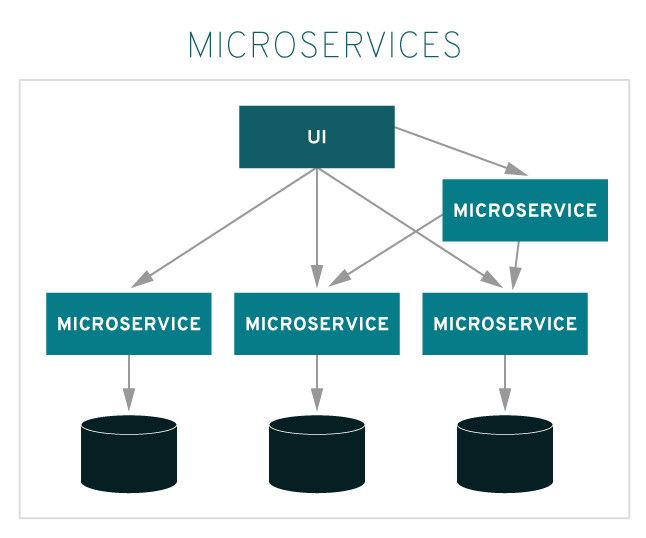
\includegraphics[width=0.45\textwidth]{monolithic-vs-microservices_altered.png}
            \caption{Structure of Microservices - [Altered] \\\textit{Source:~\cite{redhat_micro}}}\label{fig::micro}
        \end{figure}

        \subsubsection{Virtualization and Containerization}
        Virtualization is an abstraction layer. The physical hardware (called host) runs a hypervisor that allows the execution of (multiple) virtual machines (called guests) which act like a regular computer \cite{vmbasics}. This approach allows the usage of heterogeneous hardware without an impact on the guest operating systems thanks to the abstraction provided by the hypervisor. Without the need for specialized hardware and the dynamic allocation of resources, efficiency is also increased \cite{redhat_venv}. Additionally, virtual systems can be managed more easily because fundamentally they are just one big file on the host's storage device. They can be created on command, cloned and deleted without the configuration steps of a physical system. In the enterprise industry it is common to use this flexibility to start additional \ac{VM}s on high load. According to a study by the \ac{IDC} more than 80\% of datacenter workloads are virtualized \cite{virtualaddoption}. Virtualization also comes with the benefit of security. The majority of hypervisors strictly separate the host and the guest system. The guest system is not allowed to use the hosts resources and access its files unless it is explicitly configured to do so. Compromising a \ac{VM} does not affect the host or any other \ac{VM}s \cite{redhat_venv}.\newline
        Full guest virtualization emulates a complete \ac{OS}, including the kernel, system libraries and even the majority of hardware devices. This abstraction comes with a performance penalty called overhead \cite{vmbasics}. A supposedly more lightweight approach of virtualization is called containerization. Studies by Ericsson Research, Nomadic Lab \cite{ieee_perfomance} and the Zhengzhou University \cite{zhengzhou_university} conclude in fact that container based solution provide better performance especially in disk \acs{I/O} and network \acs{I/O} bound scenarios. Containerization focuses on the isolation of one application process in a virtual runtime using control groups and namespace technologies \cite{cgroups}. Unlike \ac{VM}s, system and kernel functions are not virtualized and are passed through to the host machine. The result is a reduction of overhead and the ability to run additional application instances compared to \ac{VM}s with the same amount of compute resources. Fig. \ref{fig::vm_docker} visualizes the differences between these approaches.\newline
        Apart from the performance benefits, the presumably main advantage of containers is their scalability \cite{cintainer_scale}. Which makes them an adequate fit for Microservices.

        \begin{figure}
            \centering
            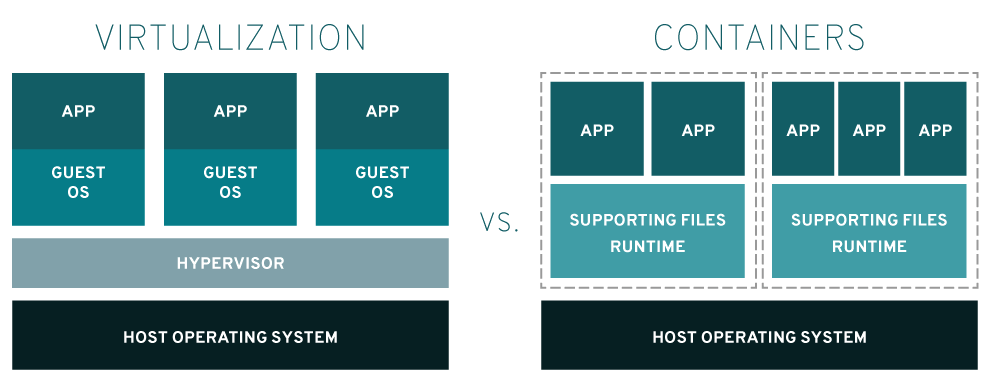
\includegraphics[width=0.9\textwidth]{docker-vm-redhat.png}
            \caption{\ac{VM}s compared to Containers \\\textit{Source:~\cite{redhat_pic}}}\label{fig::vm_docker}
        \end{figure}

        \subsubsection{Usage of Containerization in Microservices}
        As described above, microservices are small applications that communicate with each other. To follow the principles for loose coupling between the applications the communication should be performed over a programming language independent protocol. Typical \acs{IP} network protocols that are used are \ac{REST}, WebSockets or GraphQL \cite{micro}. These loose coupled applications have the advantage that they can be development simultaneously form different teams as well as upgraded and replaced independently. As a result, applications can be developed much faster and more flexibly, following the principles of agile development \cite{micro}, \cite{redhat_micro}.\newline
        The usage of containers brings this speed and flexibility even further. Containers provide a consist, isolated yet flexible runtime for applications \cite{micro_container}. Applications are packaged within known good runtimes. This reduces the setup time of the deployment and eliminate host specific errors. New application instances can be started without additional configuration. As a result of the successful concepts, tools like Docker Swarm and Kubernetes have been developed that can scale distributed applications in a managed dynamic, even automatic way.\newline
        \noindent Packaging and eventually even deploy the application introduces additional work for developers that was previously the task of the operations team. As already stated above, the developer and operations team are not separated in a DevOps culture. The new focus places value on team communication, flexibility and autonomy provided by the automation and support of as many steps as possible between the development and operation workflow \cite{effective_devops}. Eliminating manual tasks allows developers to focus on the actual application development. One of the main concepts in this process is the usage of \ac{CI} and \ac{CD} workflows.

    \subsection{\acl{CI} and \acl{CD} concepts}
    \subsection{Containerization in development environments}
\section{Concept of DevContainers}
    \subsection{Pre-requirements for DevContainers}
    \subsection{Description of a conceptual environment}
    \subsection{Available tools and resources}
    \subsection{Possible implementations approach's}
    \subsection{Strengths, weaknesses and limits}
\section{Exemplary implementation process}
    \subsection{Current state and goal}
    \subsection{Implementation approach}
    \subsection{The implementation process}
    \subsection{Encountered challenges and limits}
    \subsection{Final state}
\section{Performance evaluation and analysis}
    \subsection{Metrics and what to evaluate}
    \subsection{Evaluation and results}
    \subsection{Discussion of evaluation}
\section{Future potential and outlook}
\section{Conclusion}

\newpage
% Anhang
\lhead{Appendix}
\renewcommand{\thesubsection}{\Alph{subsection}}
\pagenumbering{Roman}
\setcounter{page}{\value{lastroman}}
\section*{Appendix}
\addcontentsline{toc}{section}{Appendix}

%Abkürzungsverzeichnis
% !TeX root = ../main.tex
\newcommand{\abbr}{Abbreviations}
\subsection{Abbreviations}
%\addcontentsline{toc}{subsection}{Abbreviations}

\begin{acronym}[1234567890]		%[längste Abkürzung]
\setlength{\itemsep}{-\parsep}	% sorgt dafür, dass das Verzeichnis kompakt dargestellt wird.

\acro{BLEST}[BLEST]{BLock ESTimation}
\acro{CWND}[CWND]{Congestion Window}
\acro{DAPS}[DAPS]{Delay-Aware Packet Scheduler}
\acro{ECF}[ECF]{Earliest Completion First}
\acro{HTTP}[HTTP]{Hypertext Transfer Protocol}
\acro{ISP}[ISP]{Internet Service Provider}
\acro{IETF}[IETF]{Internet Engineering Task Force}
\acro{LRF}[LRF]{Lowest-RTT-First}
\acro{MSS}[MSS]{Maximum Segment Size}
\acro{MPTCP}[MPTCP]{Multipath TCP}
\acro{MPTCPSW}[MPTCP\textsubscript{SW}]{MPTCP's send window}
\acro{OTIAS}[OTIAS]{Out-of-Order Transmission for In-Order Arrival Scheduler}
\acro{RR}[RR]{Round Robin}
\acro{RTT}[RTT]{Round Trip Time}
\acro{SCTP}[SCTP]{Stream Control Transmission Protocol}
\acro{sRTT}[sRTT]{Smoothed RTT}
\acro{STTF}[STTF]{Shortest Transfer Time First}
\acro{TCP}[TCP]{Transmission Control Protocol}
\acro{VoIP}[VoIP]{Voice over IP}
\end{acronym}
\newpage

%Code
% !TeX root = ../thesis_main.tex
\subsection*{Code for you}
\addcontentsline{toc}{subsection}{Code for you}
\begin{lstlisting}[frame=single, caption={DemoCode},label=code::sttf]
    int main(){
        int i;

        // Line comment.
        puts("Hello world!");

        for (i = 0; i < N; i++){
            puts("LaTeX is also great for programmers!");
        }

        return 0;
    }
\end{lstlisting}
\newpage
\listoffigures


%Bibliographie
\addcontentsline{toc}{section}{References}
\bibliographystyle{IEEEtranSA}
% \bibliographystyle{alpha}
\bibliography{bib/sources}
% !TeX root = ../main.tex
\section*{Declaration of Authorship}

\vspace{5cm}

~\\
I hereby declare that the paper submitted is my own unaided work. I assure that I wrote this paper without using any other means and sources than those specified. As well as the sources used literally or analogously taken from the sources identified as such.

\vspace{3cm}
\begin{flushright}

\rule{8cm}{0.2mm} \\
Signature (\myName)
\end{flushright}

\vspace{2cm}
\place, the \submission{}

\end{document}